\chapter{3D Segmentation}

In this chapter, we establish the task of 3D Segmentation of EM Images, attempt to train models that perform well on this task, and evaluate our results. The purpose of these experiments is not so much to achieve state-of-the-art performance on the task, but to examine the effect that increasing training data quality and reducing variance in predictions has on model performance.

\section{Task Definition}

The problem of 3D Segmentation is formulated as such: given a stack of 2-dimensional EM images generated that represent a 3-dimensional volume of tissue (i.e. the images were taken of successive physical slices of tissue), produce a segementation\footnote{A segmentation of an image or a stack of images is defined as producing a label for each pixel in the image or stack of images, where each unique label corresponds to a discrete object in the physical volume.} of the set of images that uniquely labels each discrete entity in the original volume. That is, if a tissue volume contains a neuron that passes vertically through several different slices, then the portions of each slice through which the neuron passes would be labeled with the same identifier. This problem is significantly more complicated than the boundary prediction problem stated before, because it requires an awareness of context in 3 dimensions, rather than 2. Additionally, most EM datasets are anisotropic, meaning that the resolution is not uniform in all directions (specifically, the z-direction perpendicular to the plane of each image is generally dilated). An example of a segmentation can be found in Figure \ref{fig:snemi3d_example}.

\begin{figure}[h]
    \centering
	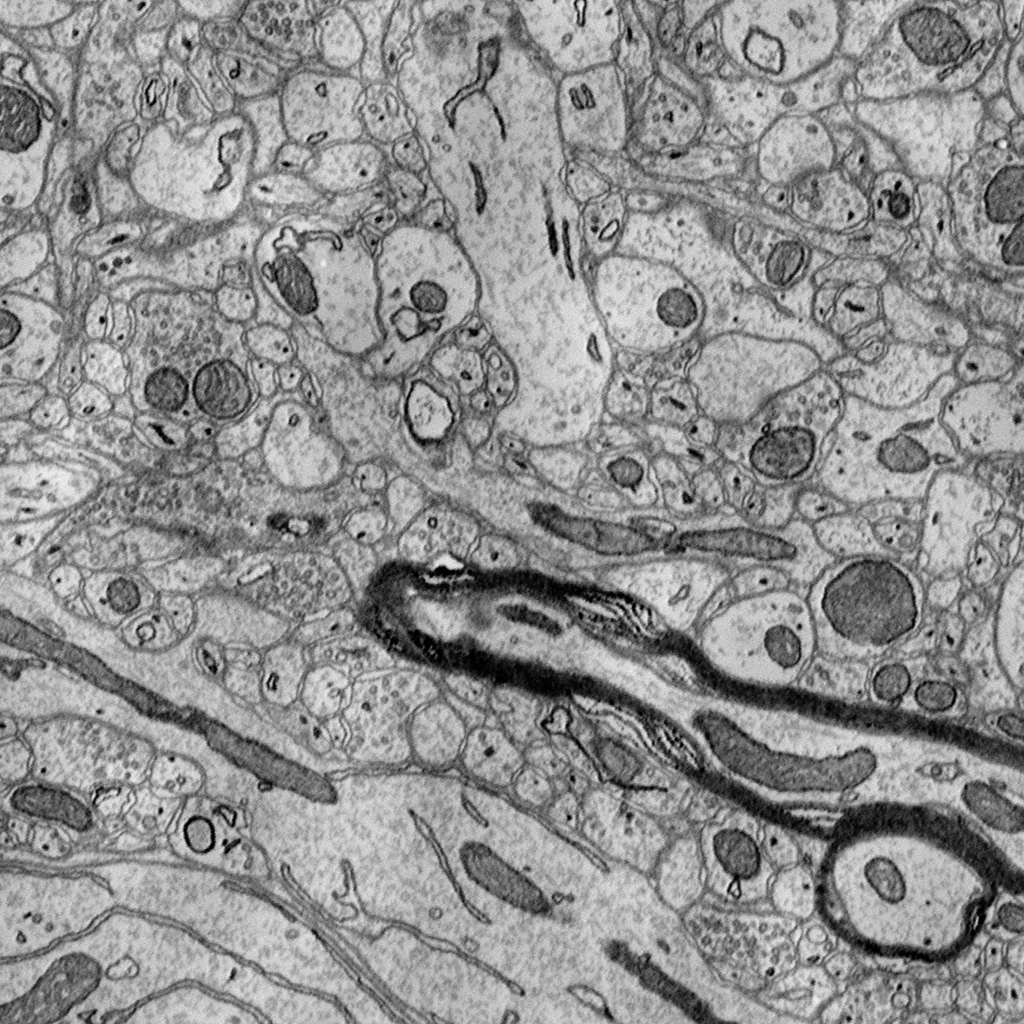
\includegraphics[width=0.33\textwidth]{img/snemi3d_raw_example}
	\hspace{1cm}
	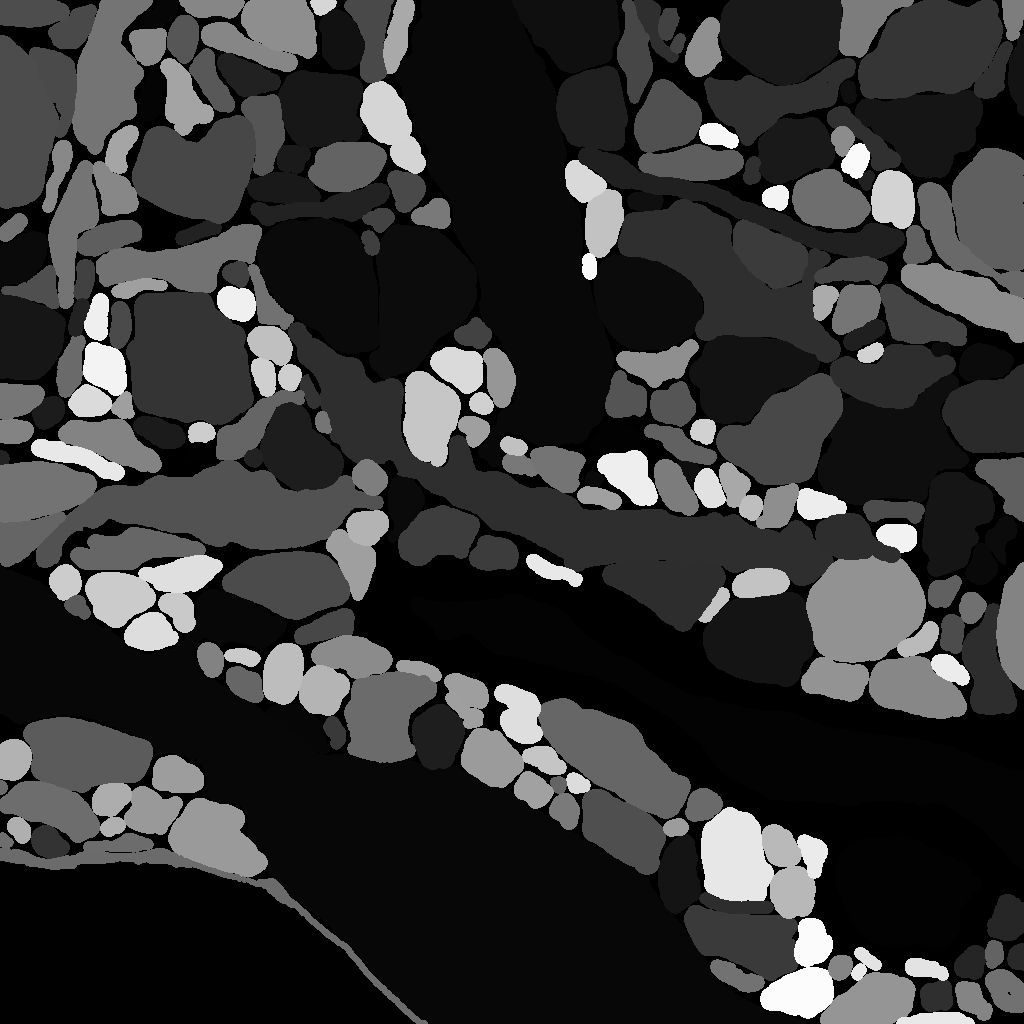
\includegraphics[width=0.33\textwidth]{img/snemi3d_label_example}
    \caption[An example of a 2D cross-section of a 3D segmentation]{An example of a 2D cross-section of a 3D segmentation. Left: one of the original images in a stack of images taken with an electron microscope. This particular example is neuron tissue taken from the common mouse in a dataset used in the ISBI 2013 EM segmentation challenge \cite{Kasthuri2015}. The resolution of each pixel is 6nm x 6nm, and each image represents a slice 30nm thick. Right: The ground truth segmentation corresponding to a segmentation of each individual object in the input image, as labeled by human experts. The labels are unique identifiers, although the border deliniation is somewhat arbitrary due to the fact that real applications of boundary detection are invariant to small differences in boundary shapes.}
    \label{fig:snemi3d_example}
\end{figure}

Trivially, the complexity of objects in 3 dimensions is potentially much greater than in two dimensions, so it makes sense that any learning method used to train a system that performs segmentation might be adept at certain types of volumetric data, and inept at others. To evaluate methods on different types of volumetric data, we selected two different challenges that provide us with samples of neural tissue that have different geometric properties, not only due to geometric differences in the underlying tissue but also because of differences in sample preparation techniques. These two challenges are the SNEMI3D Segmentation Challenge and the CREMI Segmentation Challenge.

\section{Evaluation Metrics}

Similar to the 2D Segmentation task, the two main evaluation metrics we will use for this task are Rand Score and Pixel Error. Formal definitions of both of these error metrics can be found in Appendix A. 

\begin{itemize}
\item \textbf{Rand Score}: We will use the Rand Score to determine whether or not the segmentation process correctly labels different cells as different objects. We will also look at the Rand Split Score and the Rand Merge Score, to see where the models inaccurately split and merge different regions.
\item \textbf{Pixel Error}: We will use the Pixel Error to gauge the efficacy of our models at predicting the intermediate boundary stage.
\end{itemize}

\section{Models}

We define two models for experimentation:

\begin{itemize}
	\item \textbf{VD2D-3D}: The VD2D-3D implemented for this experiment is close to the one published by Lee et. al.\cite{Lee}. It is a standard, fully-convolutional architecture that consists of two computational stages. The first stage of the net computes a series of 2D convolutions and poolings on each slice of a given sample stack, and the second stage computes a series of 3D convolutions and poolings on the entire stack. Intermediate nonlinearities are ReLU. Because the dataset is anisotropic, the effective field of view in the z direction is much smaller than in the x and y direction in terms of pixels, which is achieved through fewer z-dimensional poolings and smaller z-dimensional convolutions. The model predicts a set of 3 affinities (x, y, z) for each pixel. The effective field of view is a 85 pixel square in the x-y plane, and 7 pixels in the z direction.

	\begin{figure}
	\centering
	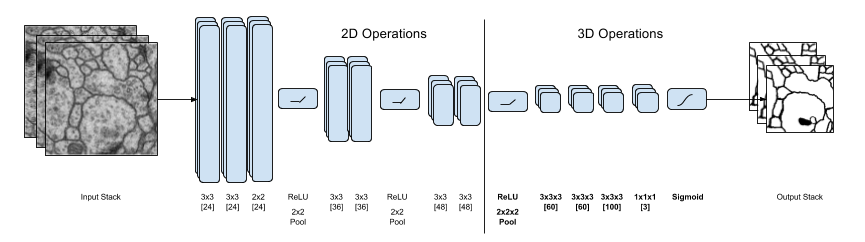
\includegraphics[width=\textwidth]{img/VD2D_3D.png}
	\caption{The VD2D-3D architecture for 3D Segmentation.}
	\label{fig:vd2d_3d}
	\end{figure}

	\item \textbf{UVR-Net}: The UVR-Net borrows concepts from the U-Net, V-Net, and Residual Nets, and is an architecture that all members of our group contributed to\cite{Ronneberger2015,He2015,Milletari2016,Cicek2016}. The structure consists of 4 "U Layers", which are pairs of down-convolutions and up-convolutions. The output of the down-convolutions skips across the net, and is concatenated to the input of the corresponding up-convolutional component (the number of feature maps of the first convolution in each "U Layer" is twice the subsequent ones). We add residual connections that skip the convolutions from the output of pooling layers, and add skip connections across the "U-Layer". After each convolution, we apply ReLU nonlinearities, except between convolutions and additions with residual connections. These modifications are all added to attempt to make the net learn first by predicting an output that looks similar to the input, and slowly eroding elements until an affinity map is left.

	\begin{figure}
	\centering
	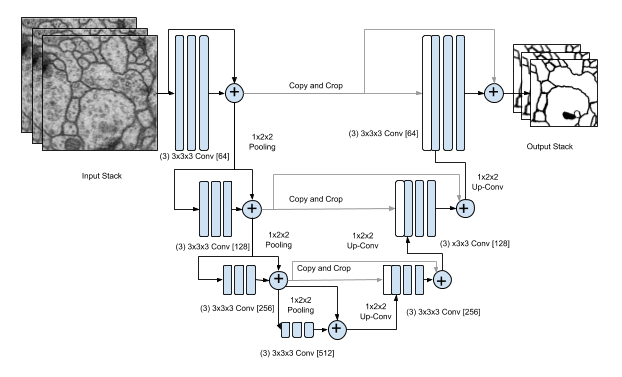
\includegraphics[width=\textwidth]{img/U-Net_3D.png}
	\caption{The UVR-Net architecture for 3D Segmentation}
	\label{fig:uvr-net}
	\end{figure}
\end{itemize}

\section{Dataset}

We will train and experiment on (4) 3D EM Datasets, taken from two different competitons: SNEMI3D and CREMI. We evaluate on 4 datasets instead of 1 to discuss the shortcomings of these models, and how training on different types of data affect performance.

The SNEMI3D Segmentation Challenge is a highly active 3D segmentation challenge (organized in advance of ISBI 2013), and provides a stack of EM images for training, along with ground truth segmentations of the EM images in 3 dimensions. The challenge website describes the training and testing data as \quotes{stacks of 100 sections from a serial section Scanning Electron Microscopy (ssSEM) data set of mouse cortex. The microcube measures 6 x 6 x 3 microns approx., with a resolution of 6x6x30 nm/pixel}\cite{Arganda-Carreras2013}. Like the ISBI 2012 dataset, the SNEMI3D dataset is anisotropic, and particularly dilated in the z-direction. Additionally, the data is from mouse cortex, rather than from \textit{Droposphilia}, and the geometry of the tissue is significantly different. 

The SNEMI3D dataset comes with a train and a test set, both of which consist of (100) 1024x1024 pixel images. The train set includes a set of labels, which represent a segmentation of the bodies in the stack. Since the test set does not include such a segmentation, we create a validation set of 25 images (25\%) which we will use to evaluate the performance of our models.

The Circuit Reconstruction from Electron Microscopy Images (CREMI) Challenge is a somewhat less-active challenge organized in advance of MICCAI 2016\cite{Funke.Jan2016}. The challenge provides three datasets for training, all of which are volumetric samples of \textit{Drosophila melanogaster}. The training and testing data are stacks of 125 sections from an ssSEM data set, with each slice having a resolution of 4x4x40nm/pixel. These datases are also anisotropic, being dilated in the z-direction. Furthermore, the types of neurons sampled are quite diverse between datasets: from visual inspection, some of the neurites in one of the datasets is much thinner than those in the others, suggesting that models might perform differently when trained/tested on these different datasets. Finally, these datasets are quite a bit noisier than ISBI or SNEMI3D: there are many more major misalignments, many patches of blur, and some slices are missing entirely. These datasets will provide a good measure of how robust our methods are to noise in volumetric data.

The three CREMI datasets (labeled CREMI A, CREMI B, and CREMI C) contain train and test sets, each of which consist of (125) 1250x1250 pixel images. The train set includes a set of labels, which represent a segmentation of the bodies in the stack. Like SNEMI3D, the test sets don't include segmentaitons, so we create validation sets from the training sets by witholding 25 slices (20\%) from each for evaluation of model performance.

\section{Training}

We train each model on each of the datasets, for a total of 8 training runs. Training was performed on a NVIDIA Titan X. We trained each net for 30000 iterations, sampling volumetric sections from each dataset that were 16 slices thick. For every model, we sought to minimize the cross entropy between the predicted affinities and the true afinnity labels, defining our loss function as:

$$\mathcal{L}(\bm{x}, \bm{y}) =-\log(\sigma(\bm{y}^{T}\bm{x}-(1-\bm{y}^{T})\bm{x}))$$
where $\sigma$ is the sigmoid function, $\bm{x}$ is the prediction, and $\bm{y}$ are the true affinites.

At each step, we executed one iteration of optimization using the Adam Optimizer, and ever 100 steps we made predictions on the validation set to see how well the model generalized.

\section{Results}


\begin{table}
	\centering
	\caption{Results of 3D Segmentation on various datasets}
	\subcaption*{SNEMI3D} 
	\begin{tabular}{lllll}
\toprule
{} & Pixel Error & Rand - Full & Rand - Merge & Rand - Split \\
\midrule
VD2D-3D &    0.102204 &    0.790909 &      0.95196 &     0.676465 \\
UVR-Net &   0.0863271 &    0.783288 &     0.993469 &     0.646511 \\
\bottomrule
\end{tabular}
 

	\subcaption*{CREMI A} 
	\begin{tabular}{lllll}
\toprule
{} &  Pixel Error &  Rand - Full &  Rand - Merge &  Rand - Split \\
\midrule
VD2D-3D &     0.098559 &     0.651105 &      0.981541 &      0.487117 \\
UVR-Net &     0.034879 &     0.576646 &      0.449545 &      0.803948 \\
\bottomrule
\end{tabular}
 

	\subcaption*{CREMI B} 
	\begin{tabular}{lllll}
\toprule
{} & Pixel Error & Rand - Full & Rand - Merge & Rand - Split \\
\midrule
VD2D-3D &    0.097363 &    0.845614 &     0.929446 &     0.775653 \\
UVR-Net &   0.0379261 &    0.846339 &     0.933393 &     0.774138 \\
\bottomrule
\end{tabular}
 

	\subcaption*{CREMI C} 
	\begin{tabular}{lllll}
\toprule
{} & Pixel Error & Rand - Full & Rand - Merge & Rand - Split \\
\midrule
VD2D-3D &     0.11817 &  0.00283098 &      0.91909 &   0.00141767 \\
UVR-Net &   0.0419219 &    0.748079 &     0.933252 &     0.624223 \\
\bottomrule
\end{tabular}
 
	
	\label{tab:3d_results}
\end{table}

\begin{figure}
\centering
\textbf{SNEMI3D} \\
\textbf{Rand Index}
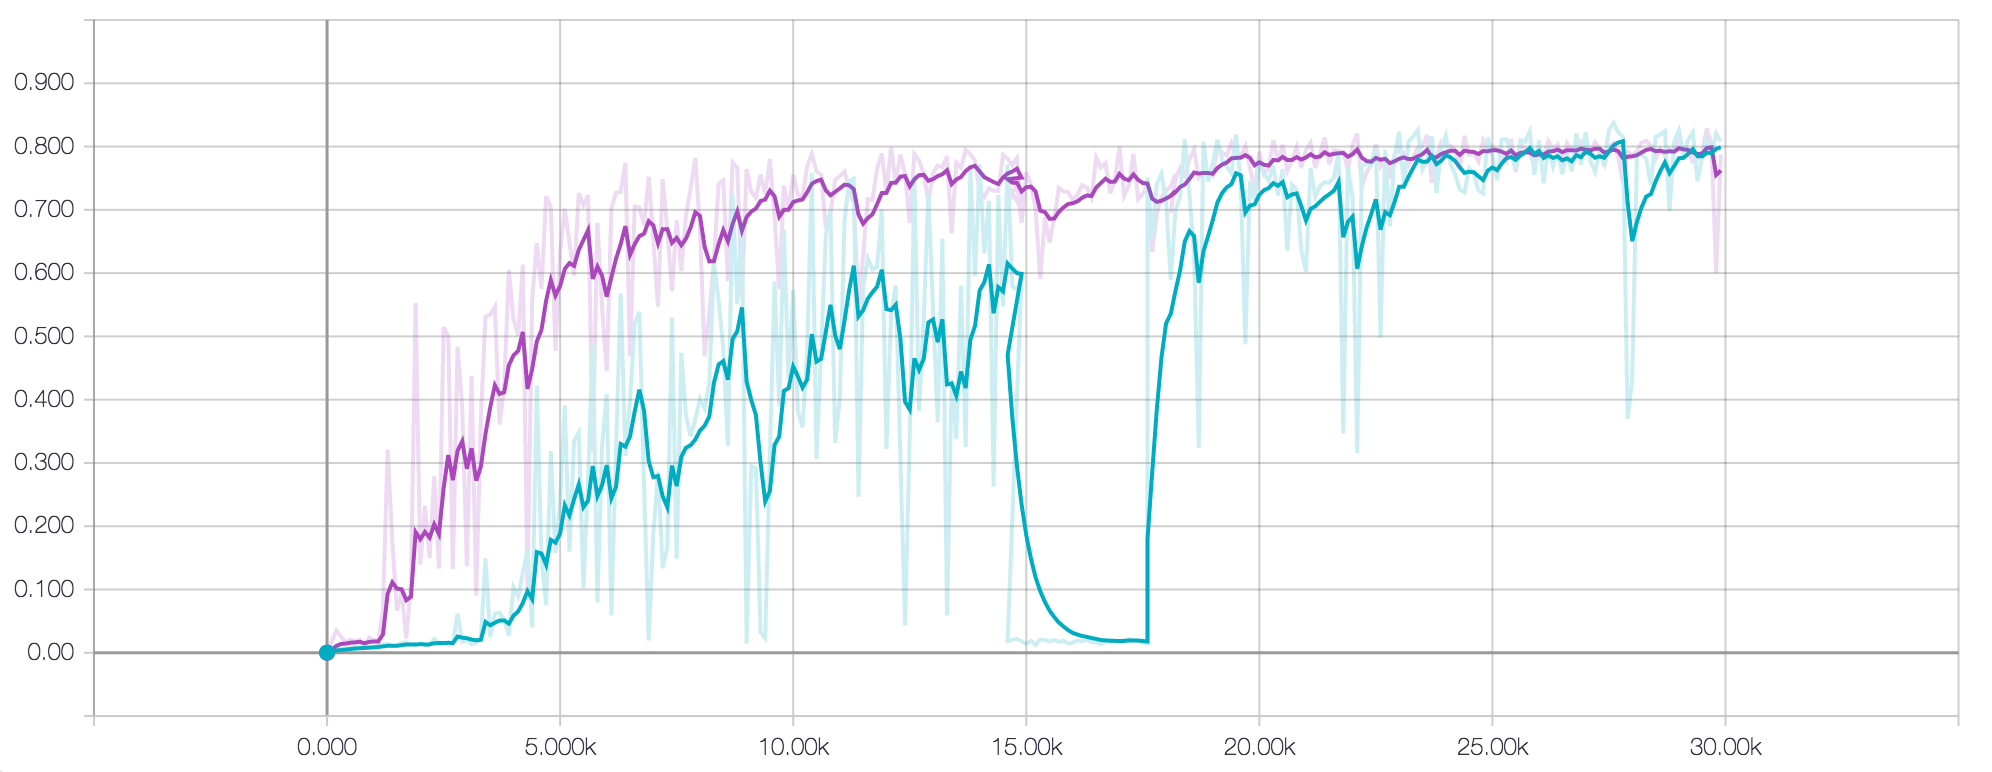
\includegraphics[width=\textwidth]{img/snemi_rand.png} \\
\textbf{Pixel Error}
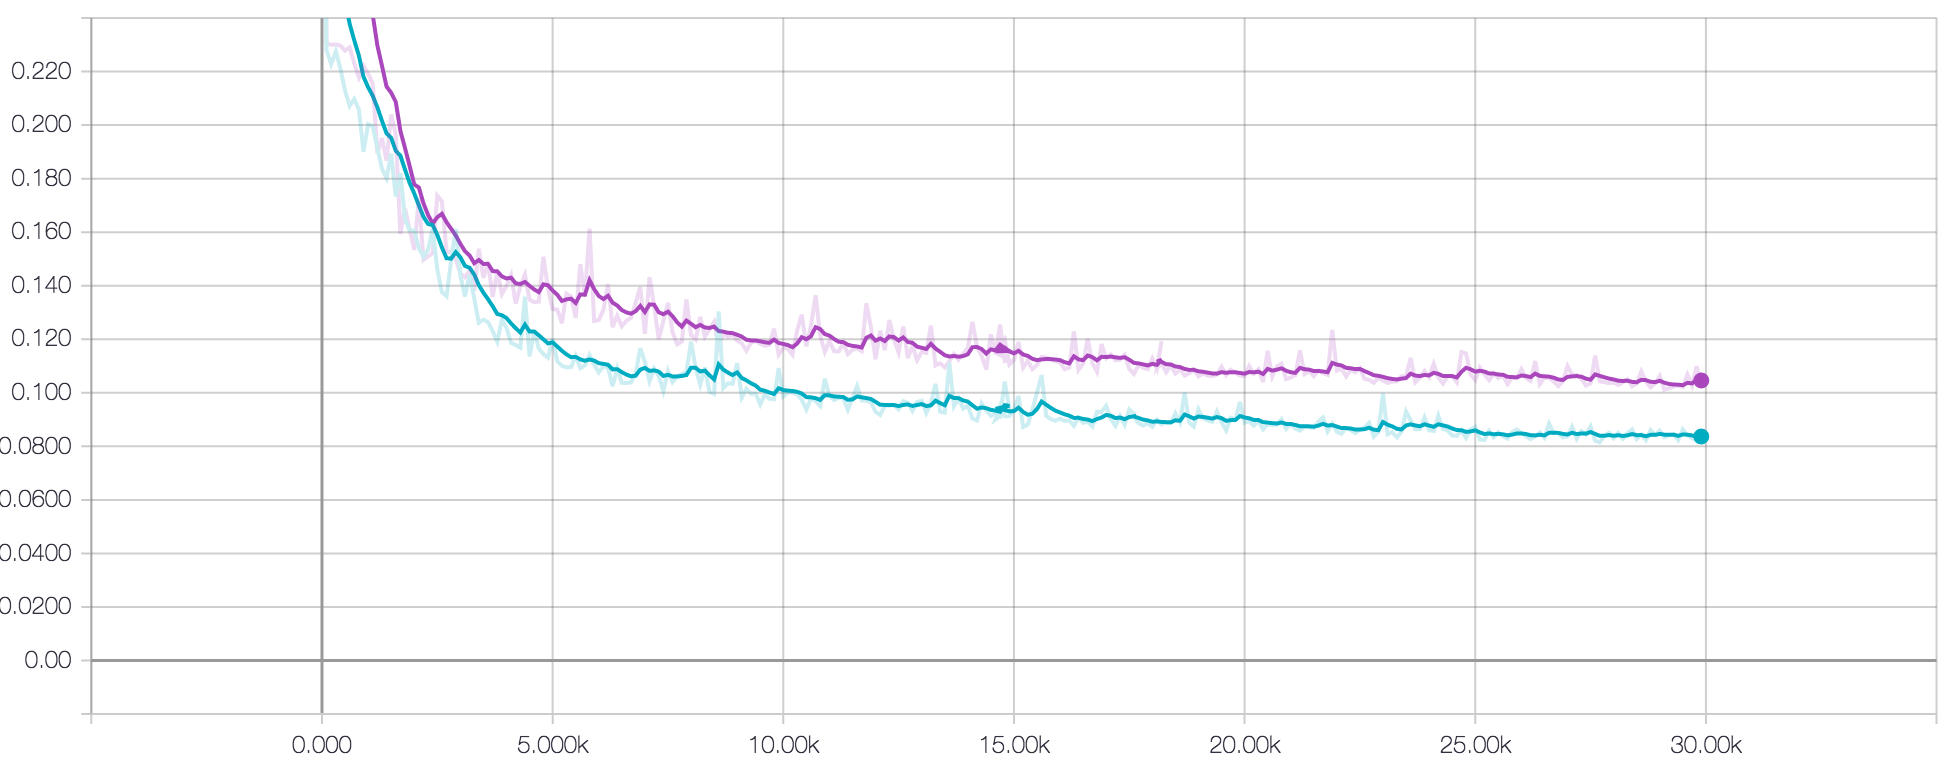
\includegraphics[width=\textwidth]{img/snemi_px_err.png}

\caption[Training curves for 3D segmentation for SNEMI3D]{Training curves, smoothed, for 3D segmentation. Top: The full Rand scores on the SNEMI3D validation set (from top: VD2D-3D, UVR-Net). Bottom: The pixel error on the SNEMI3D validation set (from top: VD2D-3D, UVR-Net). The sharp dip in the Rand Score for the UVR-Net was due to a small parameter change in validation procedure that was quickly reverted.}
\label{fig:snemi_training_curves}

\end{figure}

\begin{figure}
\centering
\textbf{CREMI A} \\
\textbf{Rand Index}
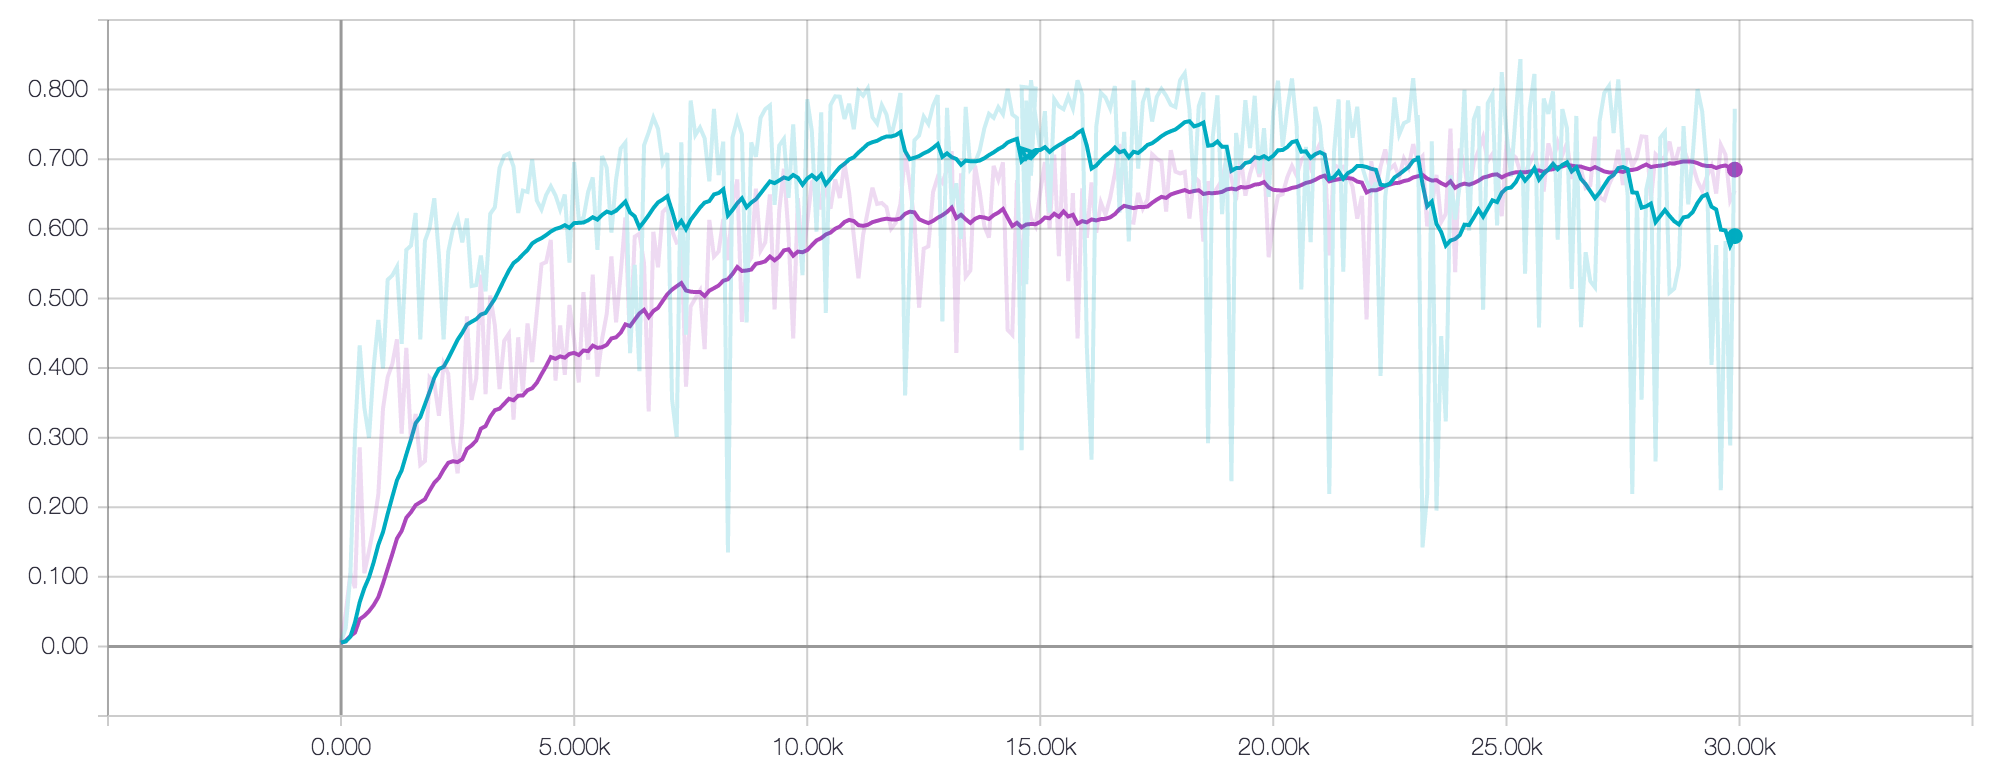
\includegraphics[width=\textwidth]{img/cremi_a_rand.png} \\
\textbf{Pixel Error}
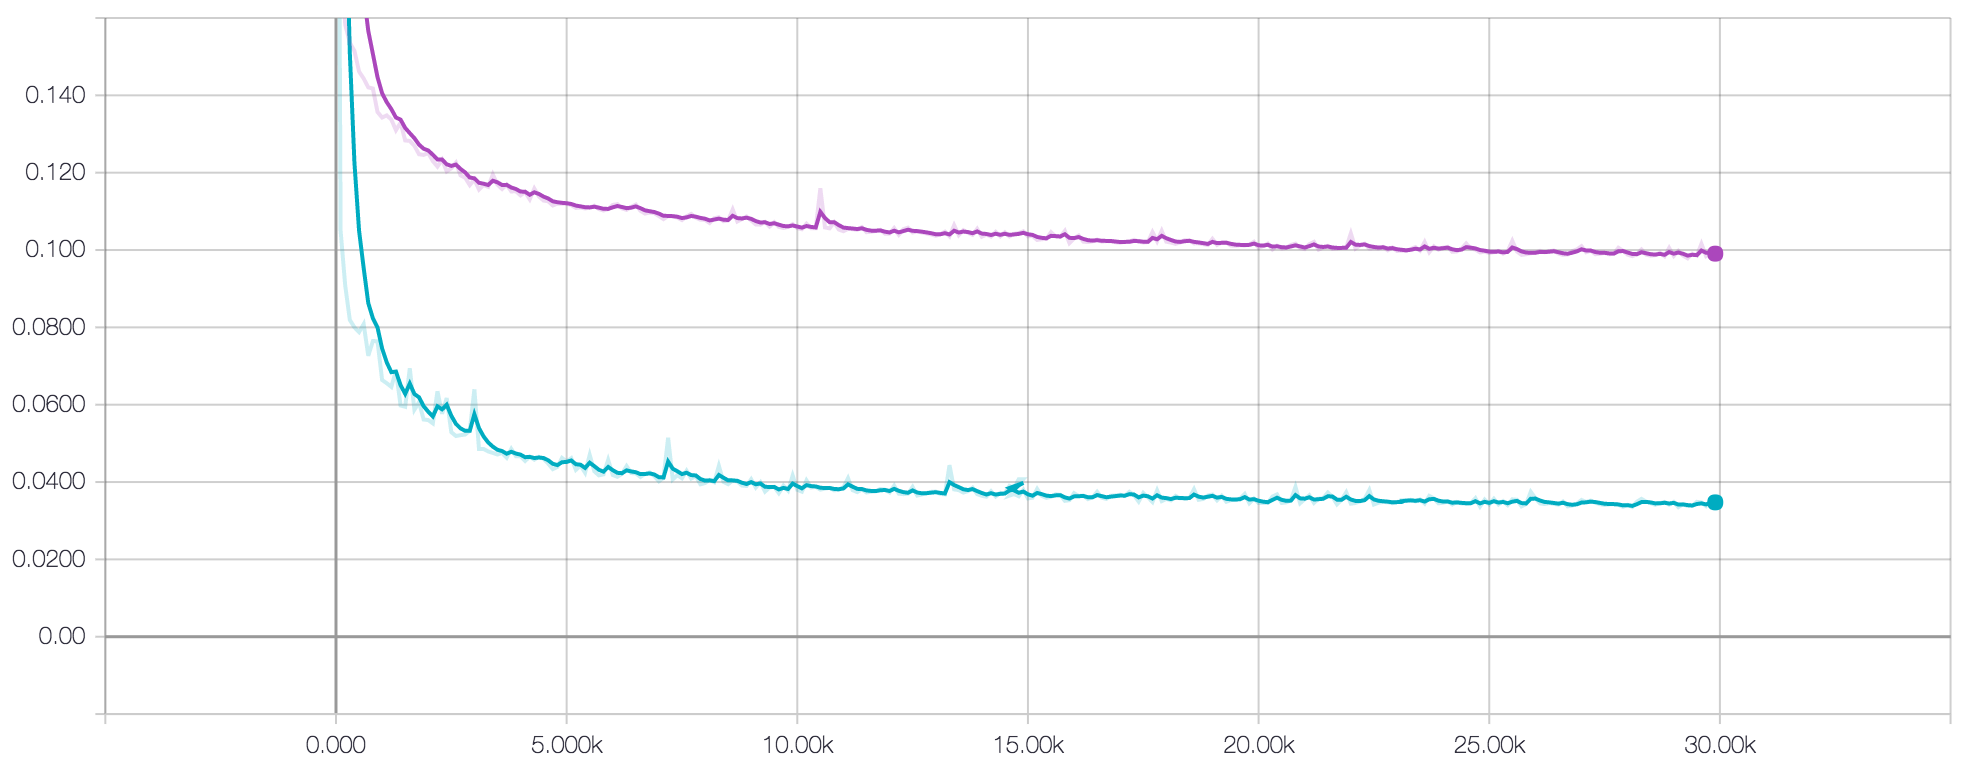
\includegraphics[width=\textwidth]{img/cremi_a_px_err.png}

\caption[Training curves for 3D segmentation for CREMI A]{Training curves, smoothed, for 3D segmentation. Top: The full Rand scores on the CREMI A validation set (from top: UVR-Net, VD2D-3D). Bottom: The pixel error on the CREMI A validation set (from top: VD2D-3D, UVR-Net).}
\label{fig:cremi_a_training_curves}

\end{figure}

\begin{figure}
\centering
\textbf{CREMI B} \\
\textbf{Rand Index}
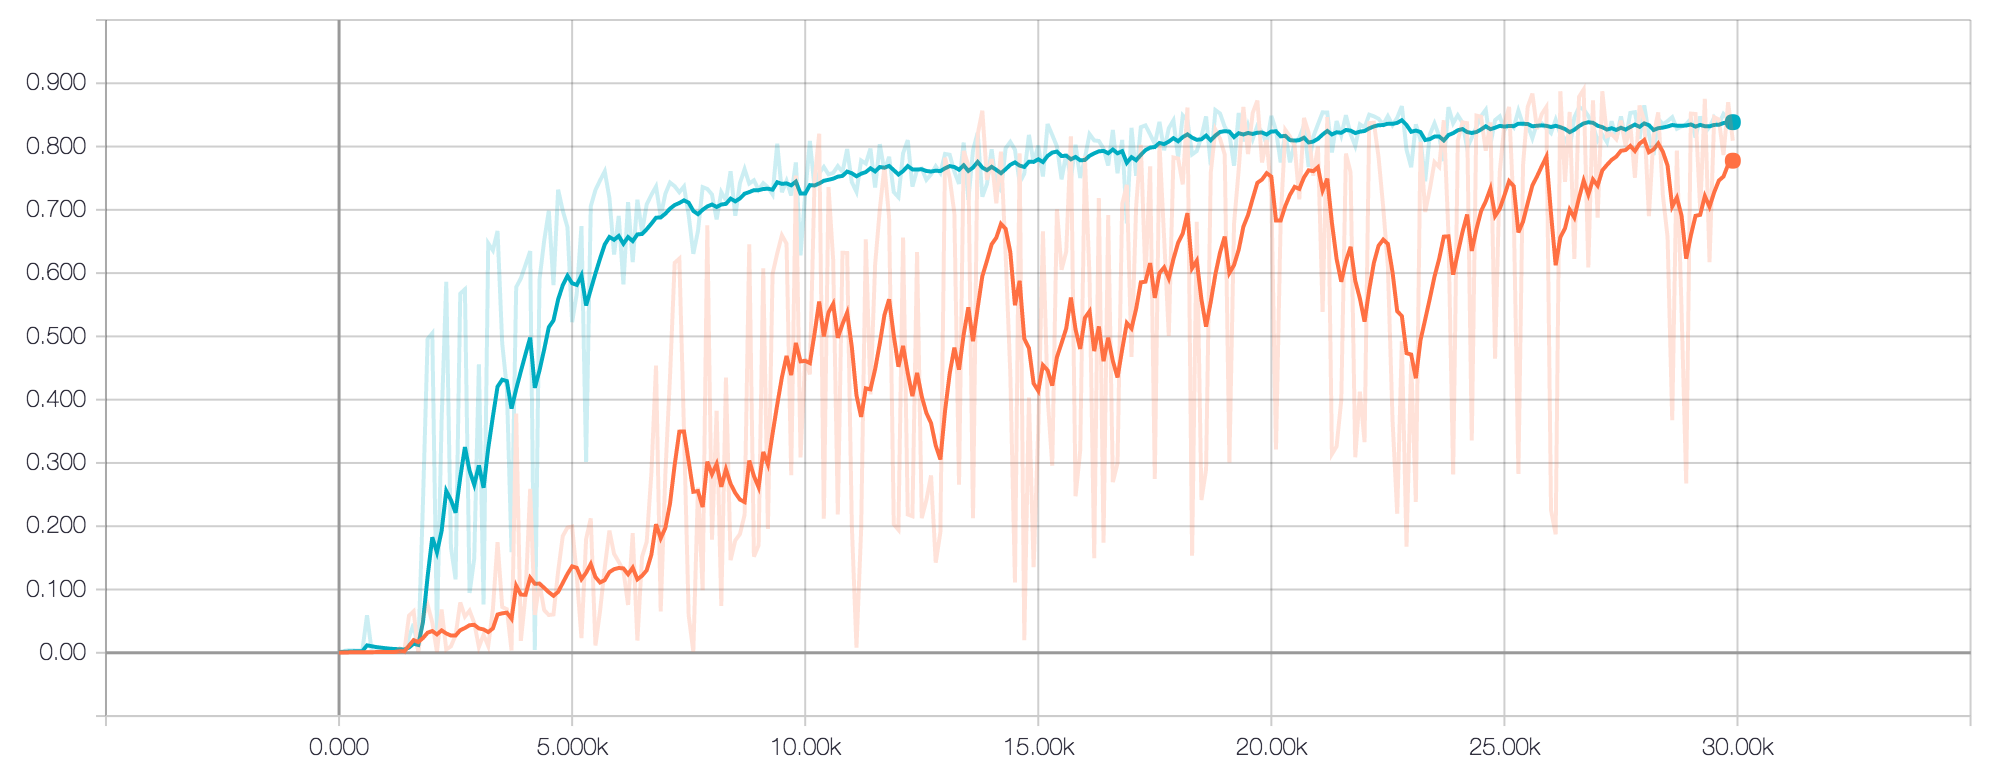
\includegraphics[width=\textwidth]{img/cremi_b_rand.png} \\
\textbf{Pixel Error}
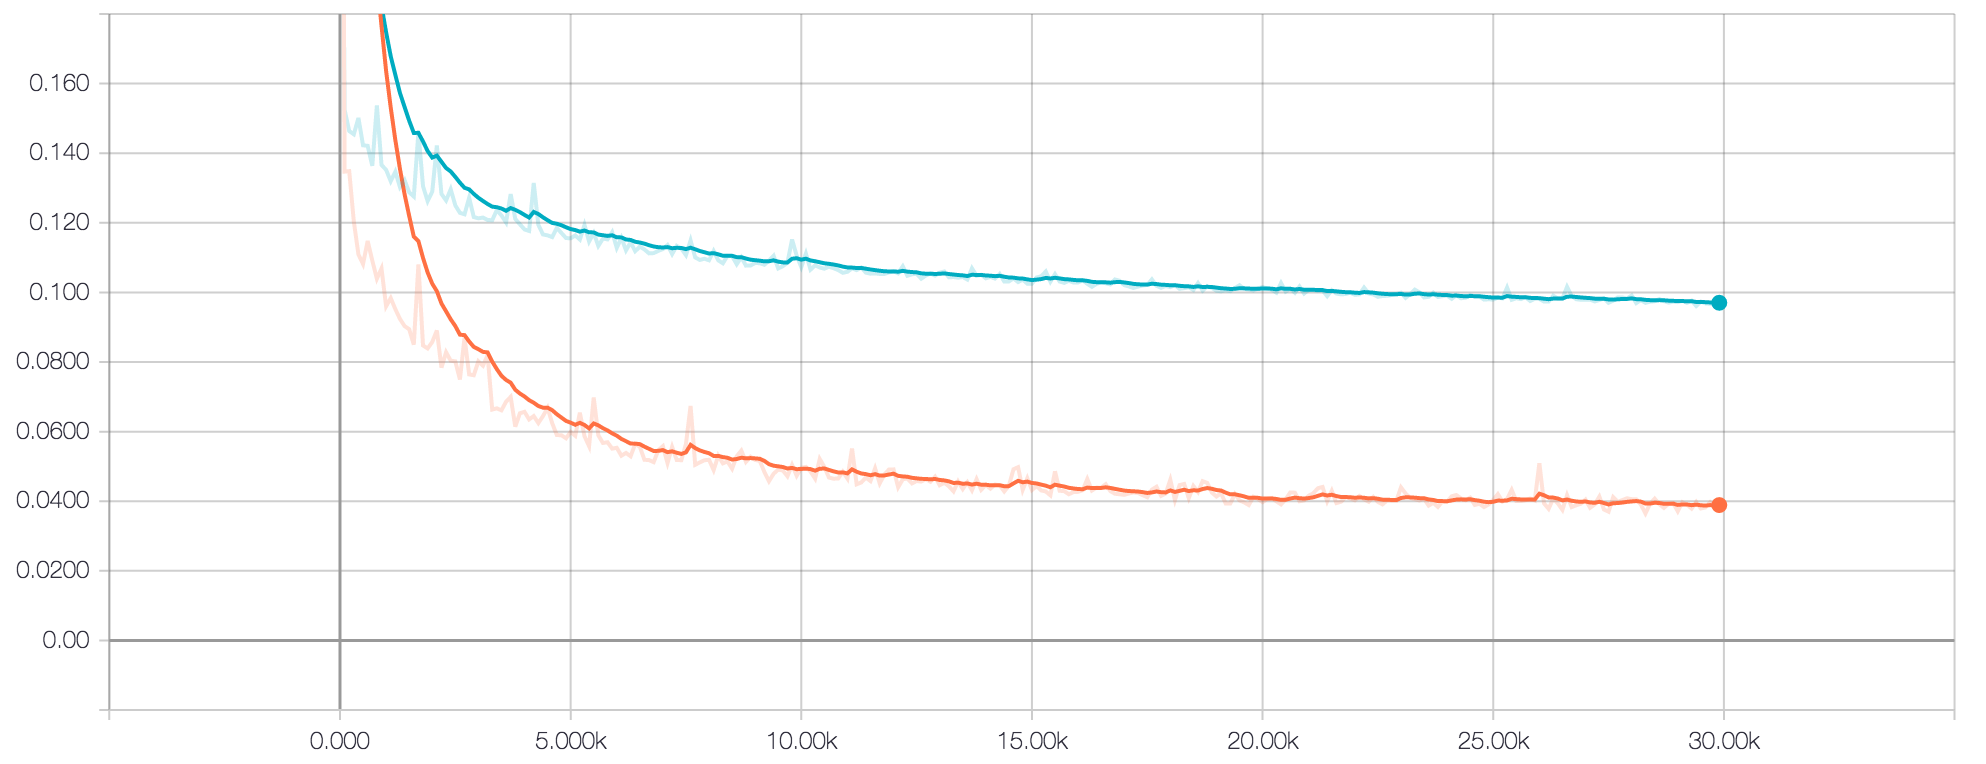
\includegraphics[width=\textwidth]{img/cremi_b_px_err.png}

\caption[Training curves for 3D segmentation for CREMI B]{Training curves, smoothed, for 3D segmentation. Top: The full Rand scores on the CREMI B validation set (from top: VD2D-3D, UVR-Net). Bottom: The pixel error on the CREMI B validation set (from top: VD2D-3D, UVR-Net).}
\label{fig:cremi_b_training_curves}

\end{figure}

\begin{figure}
\centering
\textbf{CREMI C} \\
\textbf{Rand Index}
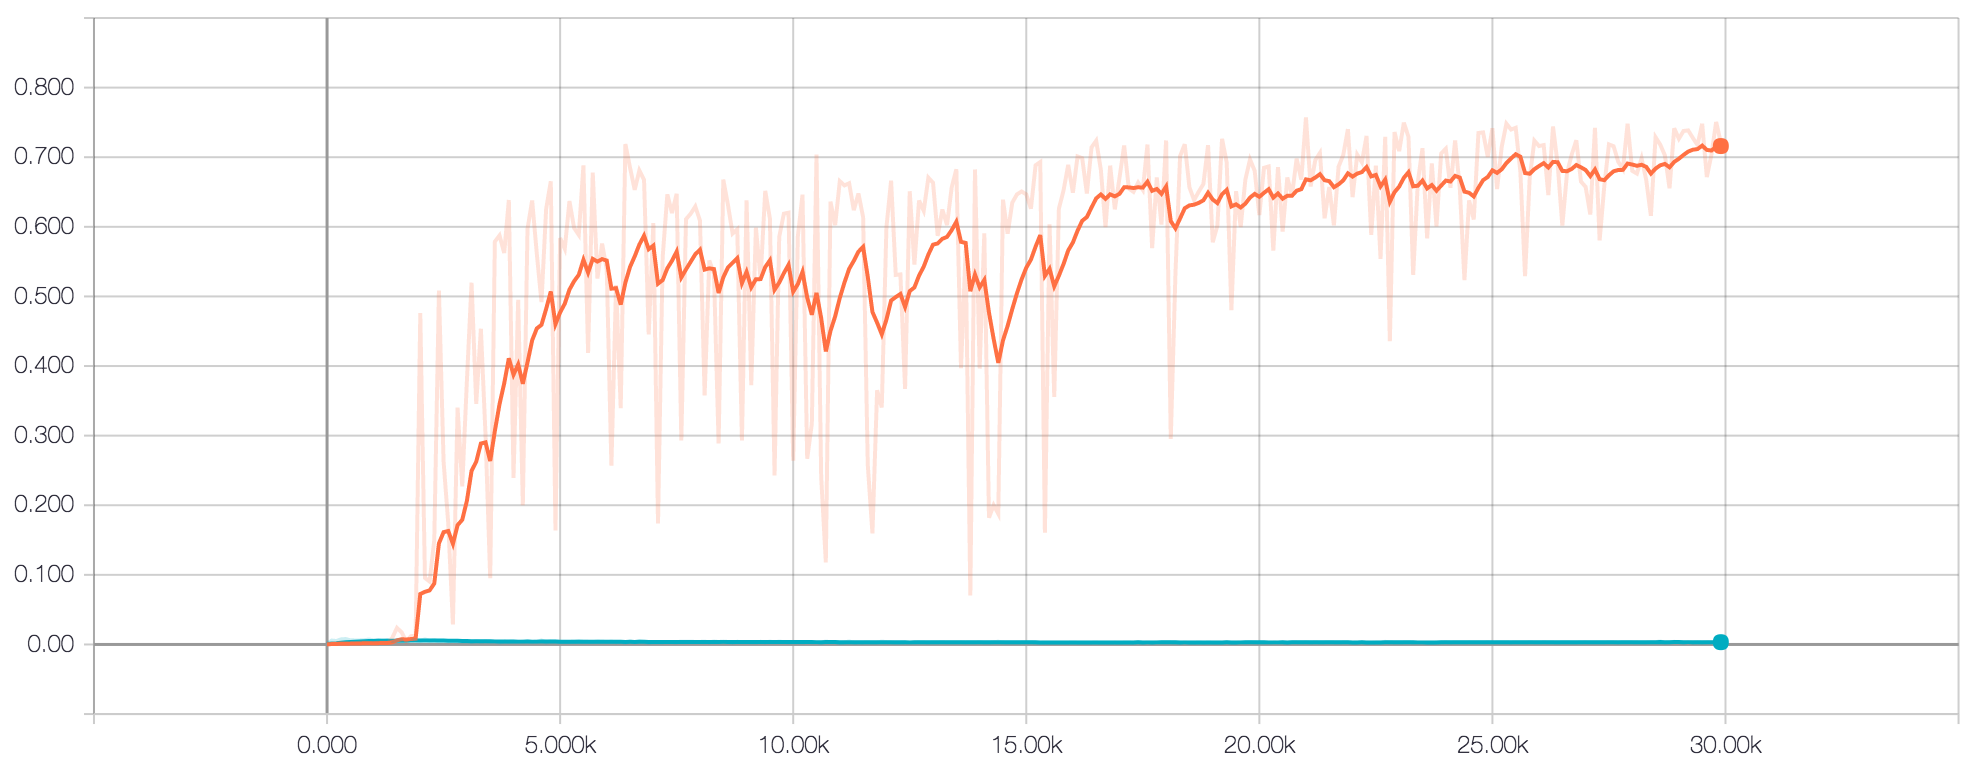
\includegraphics[width=\textwidth]{img/cremi_c_rand.png} \\
\textbf{Pixel Error}
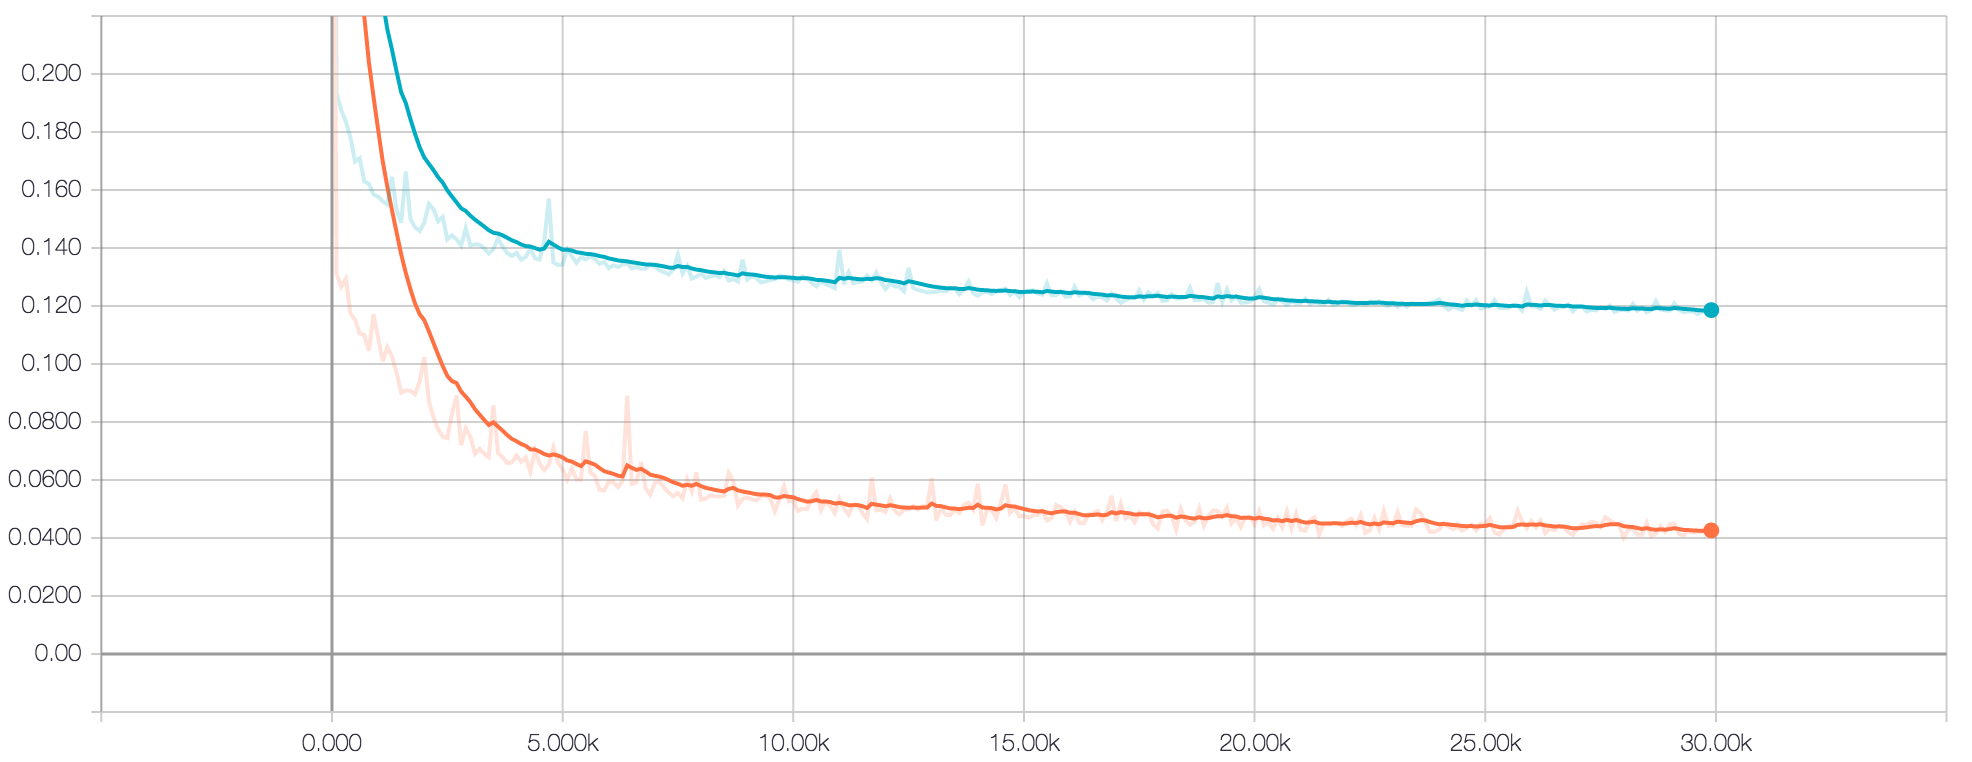
\includegraphics[width=\textwidth]{img/cremi_c_px_err.png}

\caption[Training curves for 3D segmentation for CREMI C]{Training curves, smoothed, for 3D segmentation. Top: The full Rand scores on the CREMI C validation set (from top: UVR-Net, VD2D-3D (barely pictured)). Bottom: The pixel error on the CREMI C validation set (from top: VD2D-3D, UVR-Net). The absurdly low Rand score for the VD2D-3D model might be a bit misleading; it is possible that there was a training fluke for this iteration.}
\label{fig:cremi_c_training_curves}

\end{figure}


After training, we run prediction on the validation sets for each dataset (since we don't have labels for the test set) to determine their performance. Results are numerically summarized in Table \ref{tab:3d_results}. The training graphs documenting Rand Score and Pixel Error for models training on SNEMI3D, CREMI A, CREMI B, and CREMI C can be found in Figures \ref{fig:snemi_training_curves}, \ref{fig:cremi_a_training_curves}, \ref{fig:cremi_b_training_curves}, and \ref{fig:cremi_c_training_curves}, respectively. 

We can draw several conclusions about the qualities that these models have when trained on these datasets. First, it is patently obvious that there is large variation in the training process. Sometimes, the models would train quite quickly; sometimes, they wouldn't train appropriately (in the case of VD2D-3D on CREMI C). If we were to repeat this study, we would likely train each model on each dataset multiple times with the same parameters, and take the best performing model from each set of runs. 

Second, in every setting the UVR-Net outperforms the VD2D-3D net in Pixel Error; UVR-Net consistently has substantially lower pixel error than VD2D-3D, by about the same margin in every trial. This suggests that the residual layers and skip connections built into the architecture are doing their jobs, and are reconstructing images that look a lot like the input (an affinity map should look quite like the boundaries of the input). 

Thrid, the quality of the data significantly affects the performance of these models. While some of the differences in scores can be attributed to variance in the training of the model, during the experimentation process (before results generation) it became clear that models would perform differently on different datasets. From this, we can draw the conclusion that certain datasets are "harder" than others to learn segmentatons from. What makes one dataset "harder" than another? 

In the SNEMI3D dataset, for instance, many of the objects are significantly thinner and extend longer distances across the EM slices than in the other datasets. Data quality can make a huge difference as well. The three different CREMI datasets, although taken from the same biological sample and imaged with the same process, have different properties in terms of stack quality. Visually looking at each layer of the CREMI stacks, the quality of the images varies greatly. Some of the CREMI datasets have significantly more blurred slices than others; the same goes for blemishes and cracks. CREMI C is missing a slice entirely. Individual slice artifacts may have a small impact on final metrics, but it is likely that only dataset errors affecting many slices across a dataset will have significant impact on the Rand Score of predictions. The most obvious culprit between the CREMI datasets is alignment. All three datasets are poorly aligned across the entire stack, but in terms of alignment CREMI A is worse than CREMI B and CREMI C. The Rand scores on CREMI A were also lower across all models than the other CREMI datasets. While this is not concrete evidence that the models are quite susceptible to error on poorly aligned datasets, the correlation certainly suggests that improving alignment procedures for EM datasets, or even building explicit alignment layers into models might produce better results across diverse datasets.
